%%%%%%%%%%%%%%%%%%%%%%%%%%%%%%%%%%%%%%%%%%%%%%%%%%%%%%%%%%%%%%%%%%%
%                                                                 %
%  GEANT manual in LaTeX form                                     %
%                                                                 %
%  Michel Goossens (for translation into LaTeX)                   %
%  Version 1.00                                                   %
%  Last Mod. Jan 24 1991  1300   MG + IB                          %
%                                                                 %
%%%%%%%%%%%%%%%%%%%%%%%%%%%%%%%%%%%%%%%%%%%%%%%%%%%%%%%%%%%%%%%%%%%
\Origin{R.Brun, A.McPherson}
\Submitted{29.09.83}             \Revised{18.11.93}
\Version{Geant 3.16}\Routid{GEOM130}
\Makehead{Division of a volume into a given number of cells}

\Shubr{GSDVN}{(CHNAME,CHMOTH,NDIV,IAXIS)}

Divide a volume in a given number of parts along a direction. 

\begin{DLtt}{MMMMMMMM}
\item[CHNAME] ({\tt CHARACTER*4}) a unique name for the volume to be generated
by subdivision of the mother volume;
\item[CHMOTH] ({\tt CHARACTER*4}) volume that has to be subdivided;
\item[NDIV] ({\tt INTEGER}) number of divisions into which the mother volume 
is to be divided;
\item[IAXIS] ({\tt INTEGER}) {\it axis} of the division.
\end{DLtt}

The volumes resulting from a division are true volumes in
the {\tt GEANT} sense, with the only limitation that they cannot be
positioned. They can have daughters and they can still be divided in turn.
Different divisions are distinguished by a different division number,
much the same as different copy of the same volume by the copy number.
Every operation performed on a division cell (positioning or further division),
is automatically propagated to all divisions cells of the same mother.

The kind of the division is indicated by the {\tt IAXIS} argument. 
The
allowed values of {\tt IAXIS} and the resulting divisions are shown in
figs. \ref{fg:geom130-1}, \ref{fg:geom130-2}, \ref{fg:geom130-3}, 
\ref{fg:geom130-4}, where the pictures in the first column correspond to 
an {\tt IAXIS} value equal to 1, the second column to {\tt IAXIS} = 2, 
and the third column to {\tt IAXIS} = 3 respectivly.
The
basic constraint imposed by the {\tt GEANT} geometry is that the result
of a division is a volume which can be described in terms of the basic 
shapes.

The local coordinate system of the divisions is parallel to the
system of the mother in case of divisions obtained by parallel planes or
concentric divisions. In the case of parallel axes the coordinate system
is shifted so that it is in the centre of the division.
In case of $\phi$ divisions produced by planes
passing through the axis of a volume with axial symmetry ({\tt TUBE, TUBS,
CONE, CONS, PGON, PCON, SPHE}), the local coordinate systems will be 
rotated so that the x axis passes through the centre of the division.

This routine allows the user to generate a large number of identical
volumes filling a defined volume. The material of the slices is inherited
from the mother.

It may happen that the different divisions of a volume have different
dimensions. In this case, if a volume has to be positioned in each division, 
its dimensions must be different according to the division number. This can
be obtained in some special cases giving to the dimension of the
volume which has to vary in order to fit into the different mothers,
the value of -1 in the call to
\Rind{GSVOLU} which defines it. As explained in {\tt [GEOM050]}, {\tt GEANT}
will take care to assign to this dimension the maximum value in order to
fill the current mother.

What can be done with division can be done also, in most cases, explicitly
positioning all the copies. Users must be aware, however, that divisions
offer the best performance in tracking of all {\tt GEANT} geometrical
constructs, and they should be used instead of positioning whenever
possible in the definition of objects.

\newpage
\begin{figure}[hbt]
      \centering
      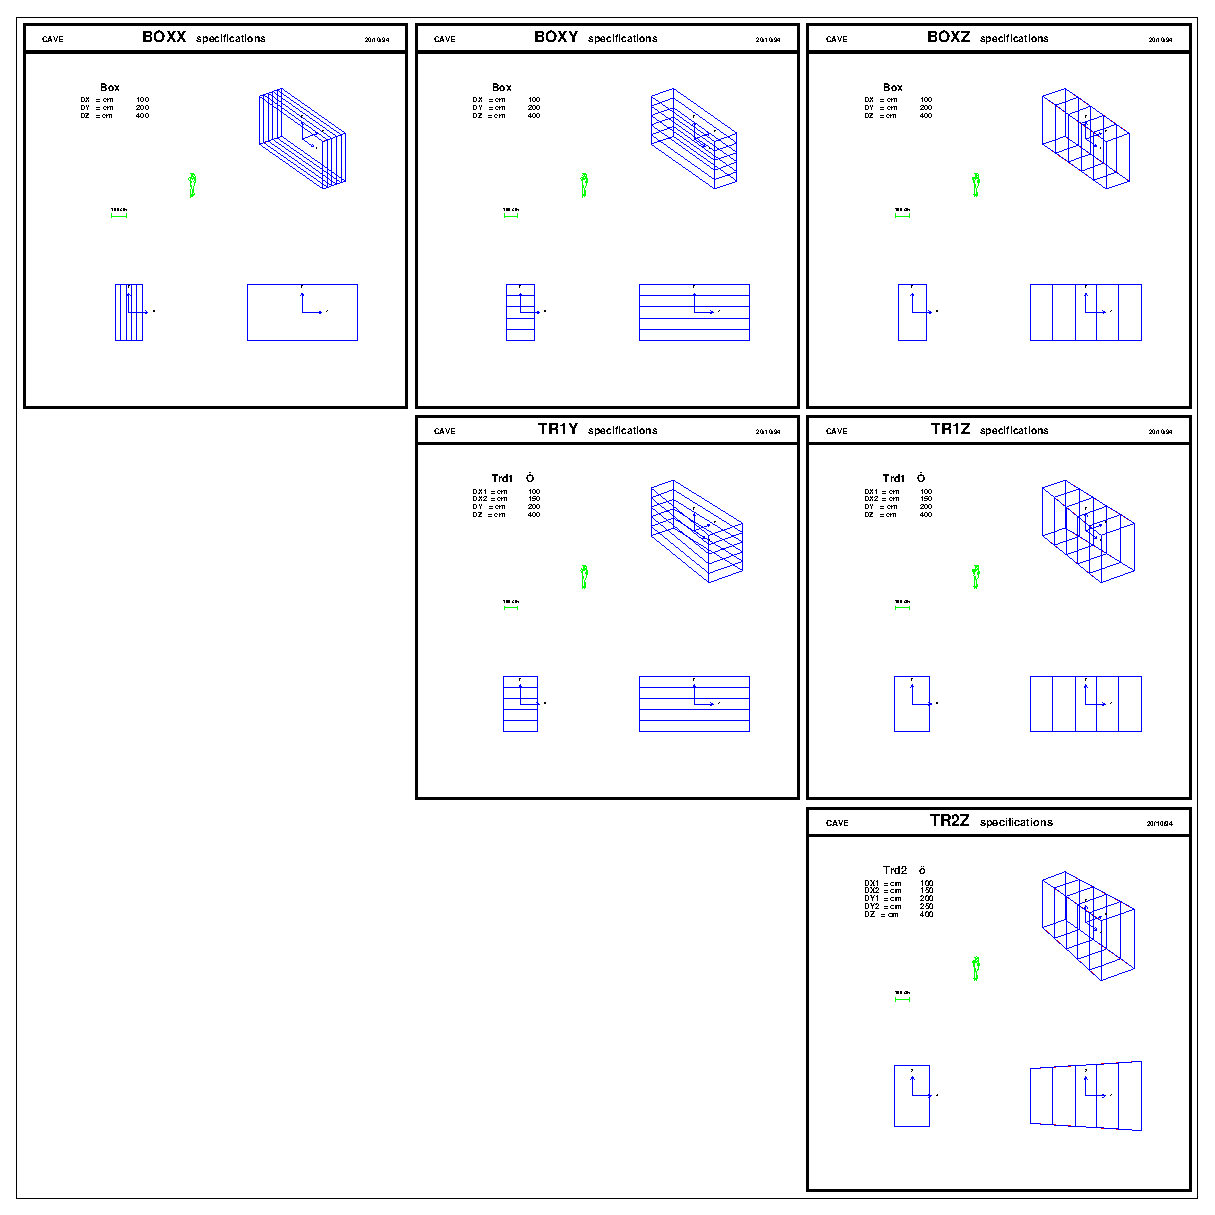
\epsfig{file=eps/geom130-1.eps,width=16cm}
      \caption{shapes {\tt BOX, TRD1, TRD2}}
      \label{fg:geom130-1}
\end{figure}
\newpage
\begin{figure}[hbt]
      \centering
      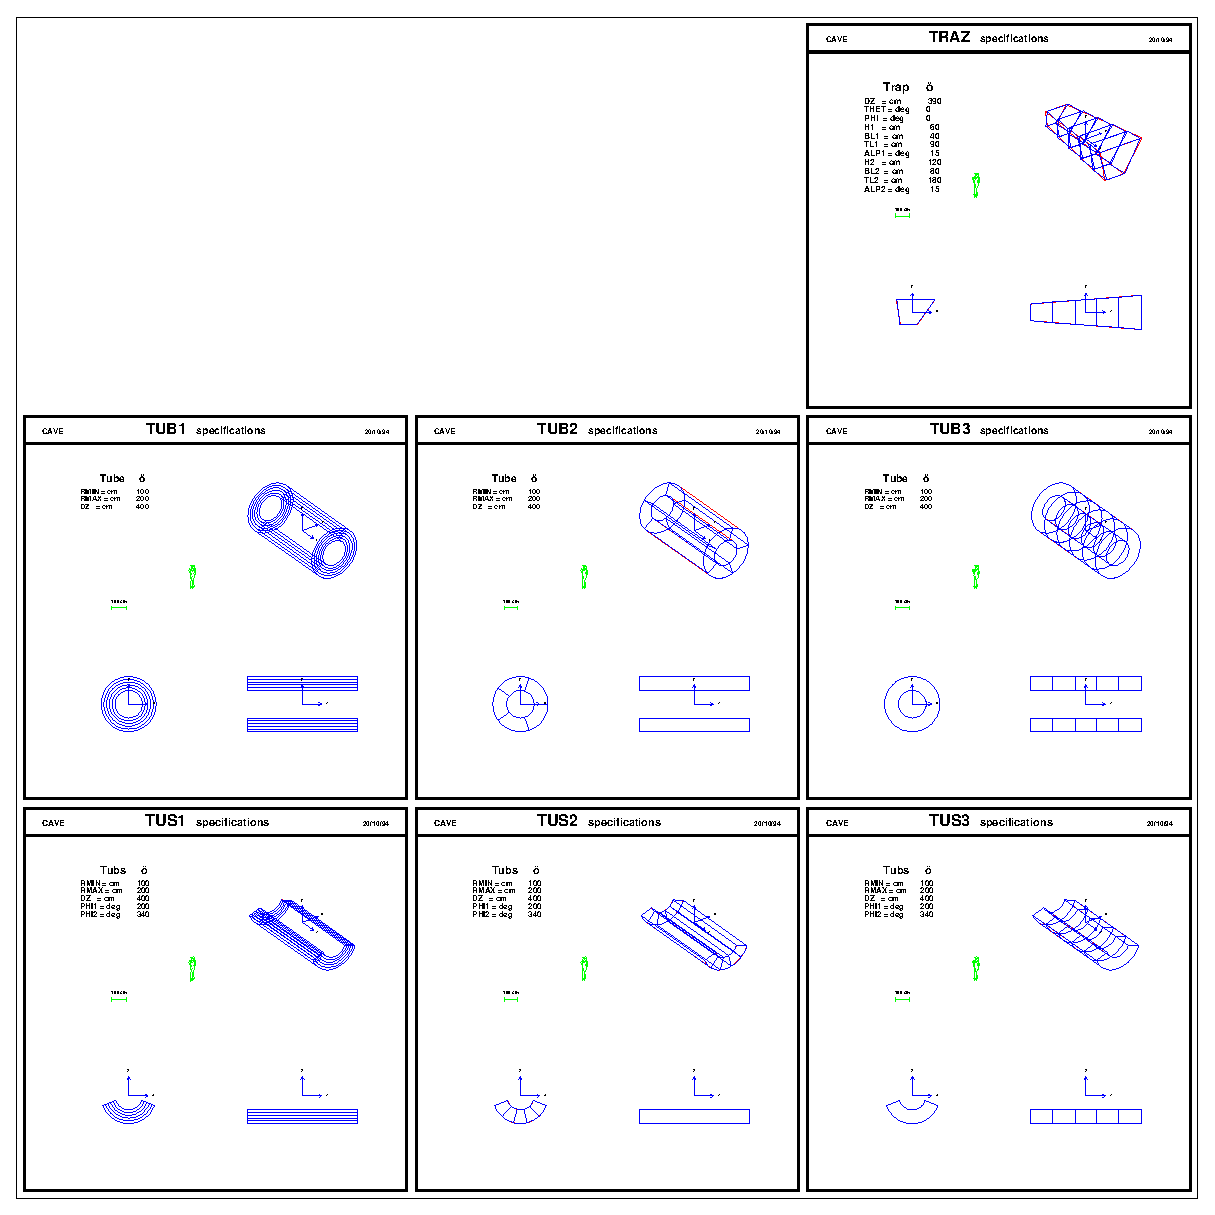
\epsfig{file=eps/geom130-2.eps,width=16cm}
      \caption{shapes {\tt TRAP, TUBE, TUBS}}
      \label{fg:geom130-2}
\end{figure}
\newpage
\begin{figure}[hbt]
      \centering
      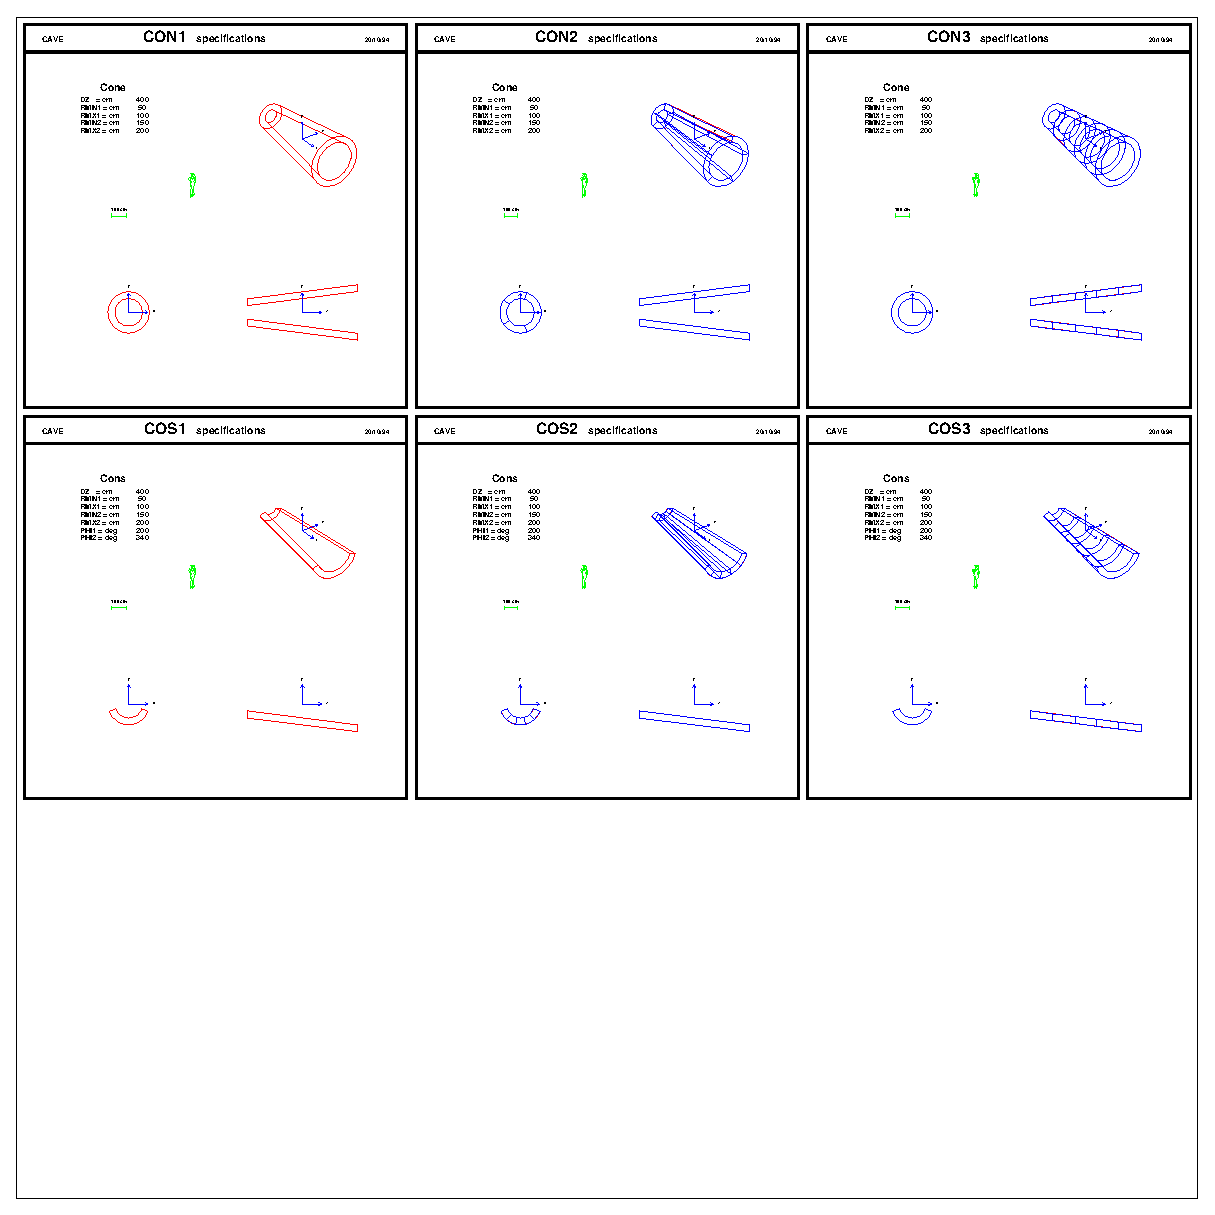
\epsfig{file=eps/geom130-3.eps,width=16cm}
      \caption{shapes {\tt CONE, CONS}}
      \label{fg:geom130-3}
\end{figure}
\newpage
\begin{figure}[hbt]
      \centering
      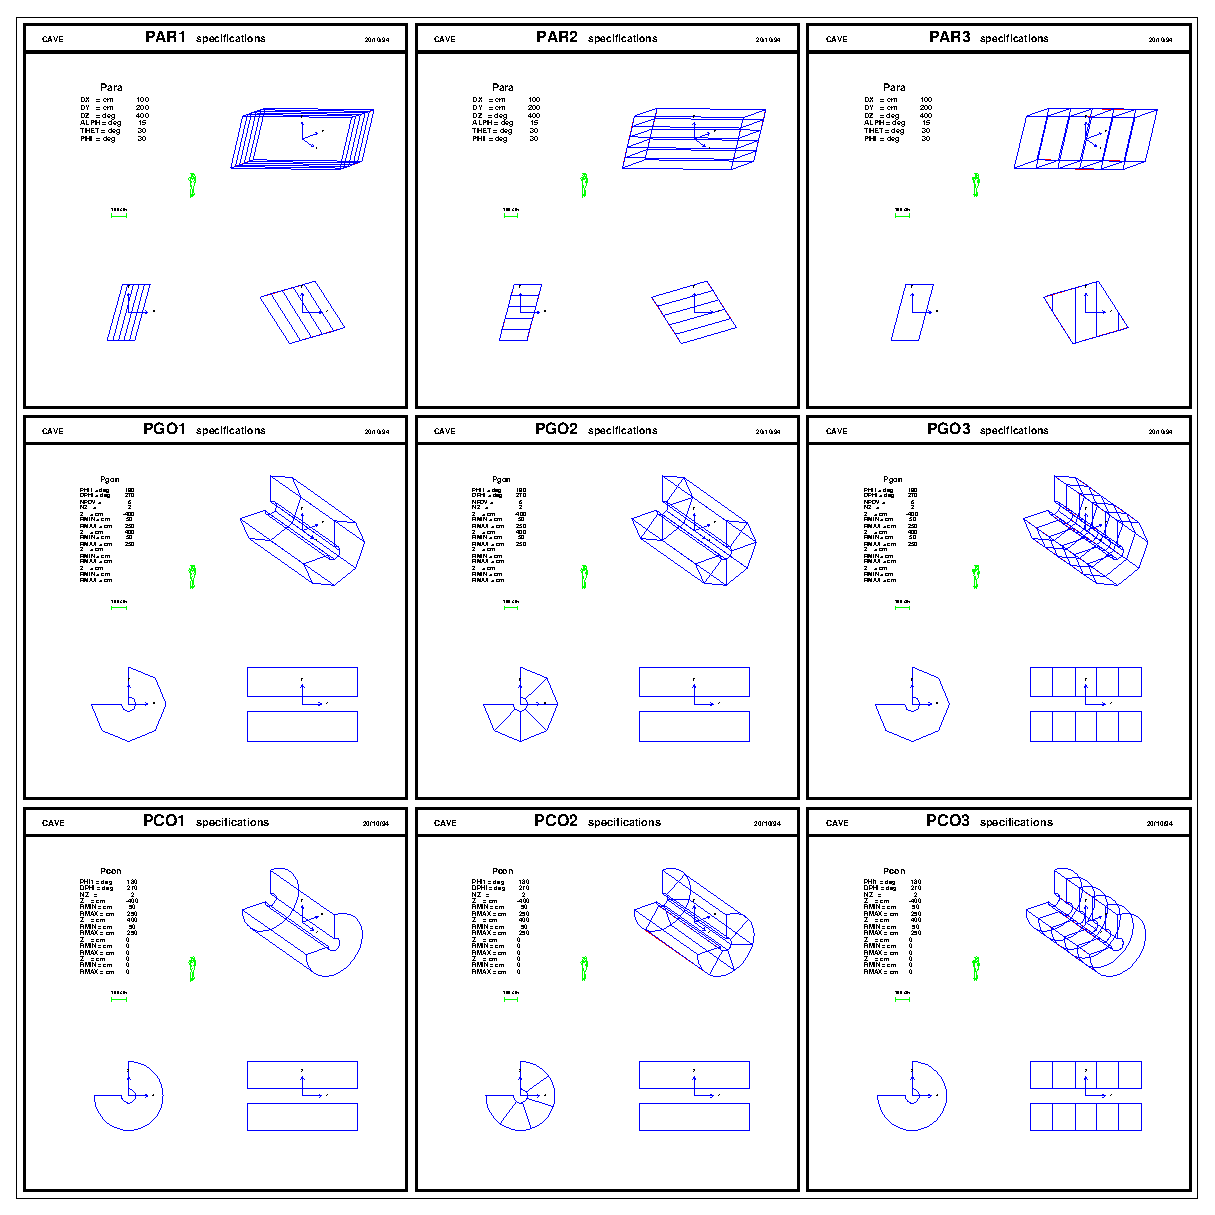
\epsfig{file=eps/geom130-4.eps,width=16cm}
      \caption{shapes {\tt PARA, PGON, PCON}}
      \label{fg:geom130-4}
\end{figure}
